\listfiles

\documentclass[a4paper,ngerman,12pt,bibtotoc]{scrartcl}

\usepackage[utf8]{inputenc}

\usepackage[ngerman]{babel}
\addto\captionsngerman{\renewcommand\tablename{Tafel}}

\usepackage{amsmath, amsthm, amssymb, stmaryrd, color, graphicx, mathtools}
\usepackage{setspace}
\usepackage{bussproofs}
\usepackage{array}
\usepackage{booktabs}
\usepackage{comment}
\usepackage{textcomp}
\usepackage{stmaryrd}

\usepackage[protrusion=true,expansion=true]{microtype}

\usepackage{lmodern}
\usepackage{tabto}

\usepackage[backend=bibtex,style=alphabetic]{biblatex}
\usepackage[babel]{csquotes}
\bibliography{literatur}

\usepackage{titling}

\usepackage[all]{xy}

\usepackage[colorlinks=true, linkcolor=blue, urlcolor=blue, citecolor=blue]{hyperref}
\usepackage{cleveref}			%Referenzen mit Name


\usepackage{algorithm}
\usepackage{algpseudocode}
\algrenewcommand{\algorithmiccomment}[1]{\hskip3em$\slash\slash$ #1}
\newcommand{\LineFor}[2]{\State\algorithmicfor\ {#1}\ \algorithmicdo\ {#2} \algorithmicend\ \algorithmicfor}


\setlength\parskip{\medskipamount}
\setlength\parindent{0pt}

\theoremstyle{definition}
\newtheorem{defn}{Definition}[section]
\newtheorem{axiom}[defn]{Axiom}
\newtheorem{bsp}[defn]{Beispiel}

\theoremstyle{plain}

\newtheorem{prop}[defn]{Proposition}
\newtheorem{motto}[defn]{Motto}
\newtheorem{ueberlegung}[defn]{Überlegung}
\newtheorem{lemma}[defn]{Lemma}
\newtheorem{kor}[defn]{Korollar}
\newtheorem{hilfsaussage}[defn]{Hilfsaussage}
\newtheorem{satz}[defn]{Satz}

\theoremstyle{remark}
\newtheorem{erin}[defn]{Erinnerung}
\newtheorem{bem}[defn]{Bemerkung}
\newtheorem{beob}[defn]{Beobachtung}
\newtheorem{aufg}[defn]{Aufgabe}

\clubpenalty=10000
\widowpenalty=10000
\displaywidowpenalty=10000

\newcommand{\ZZ}{\mathbb{Z}}
\newcommand{\QQ}{\mathbb{Q}}
\newcommand{\RR}{\mathbb{R}}
\newcommand{\CC}{\mathbb{C}}
\newcommand{\NN}{\mathbb{N}}
\newcommand{\PP}{\mathbb{P}}
\newcommand{\Ic}{\mathcal{I}}
\newcommand{\Jc}{\mathcal{J}}
\newcommand{\Hc}{\mathcal{H}}
\newcommand{\Tc}{\mathcal{T}}
\newcommand{\Sc}{\mathcal{S}}
\newcommand{\Oc}{\mathcal{O}}


\newcommand{\Hom}{\mathrm{Hom}}
\newcommand{\id}{\mathrm{id}}
\newcommand{\Id}{\mathrm{Id}}

\newcommand{\OPT}{\mathrm{OPT}}
\newcommand{\MST}{\mathrm{MST}}

\newcommand{\TSP}{\textbf{TSP}}
\newcommand{\HomTSP}{\textbf{HomTSP}}
\newcommand{\HetTSP}{\textbf{HetTSP}}
\newcommand{\CVRP}{\textbf{CVRP}}
\newcommand{\HetCVRP}{\textbf{HetCVRP}}


\renewcommand*\theenumi{\alph{enumi}}
\renewcommand{\labelenumi}{(\theenumi)}

\setcounter{tocdepth}{2}

\newenvironment{indentblock}{%
	\list{}{\leftmargin\leftmargin}%
	\item\relax
}{%
\endlist
}



\begin{document}
	\author{Lukas Graf}
	\date{Letzte Aktualisierung: \today}
	
	\selectlanguage{ngerman}
	\thispagestyle{empty}
	
	
	\begin{titlepage}\center
	\textsc{\LARGE Universität Augsburg}\\[1.5cm]
	
	\textsc{\Large Institut für Mathematik}\\[2.5cm]
	
	% Title
	{\Large Seminar\glqq ausarbeitung\grqq \\[1cm]}
	zu einem Vortrag im Seminar Spieltheorie und Approximationsalgorithmen im SS 2016 zum Thema\\[1.5cm]
	{\huge Capacitated Vehicle Routing with Non-Uniform Speeds}
		
	
	\vfill
	
	% Author and supervisor
	\begin{minipage}{0.4\textwidth}
		\begin{flushleft} \large
			\emph{Zusammengestellt:}\\
			Lukas \textsc{Graf}
		\end{flushleft}
	\end{minipage}
	\begin{minipage}{0.4\textwidth}
		\begin{flushright} \large
			\emph{Betreut von:} \\
			M. Sc. Manuel \textsc{Surek},\\Prof. Dr. Tobias \textsc{Harks}
		\end{flushright}
	\end{minipage}
	
	\end{titlepage}
	
	\section{Problemübersicht}
	
		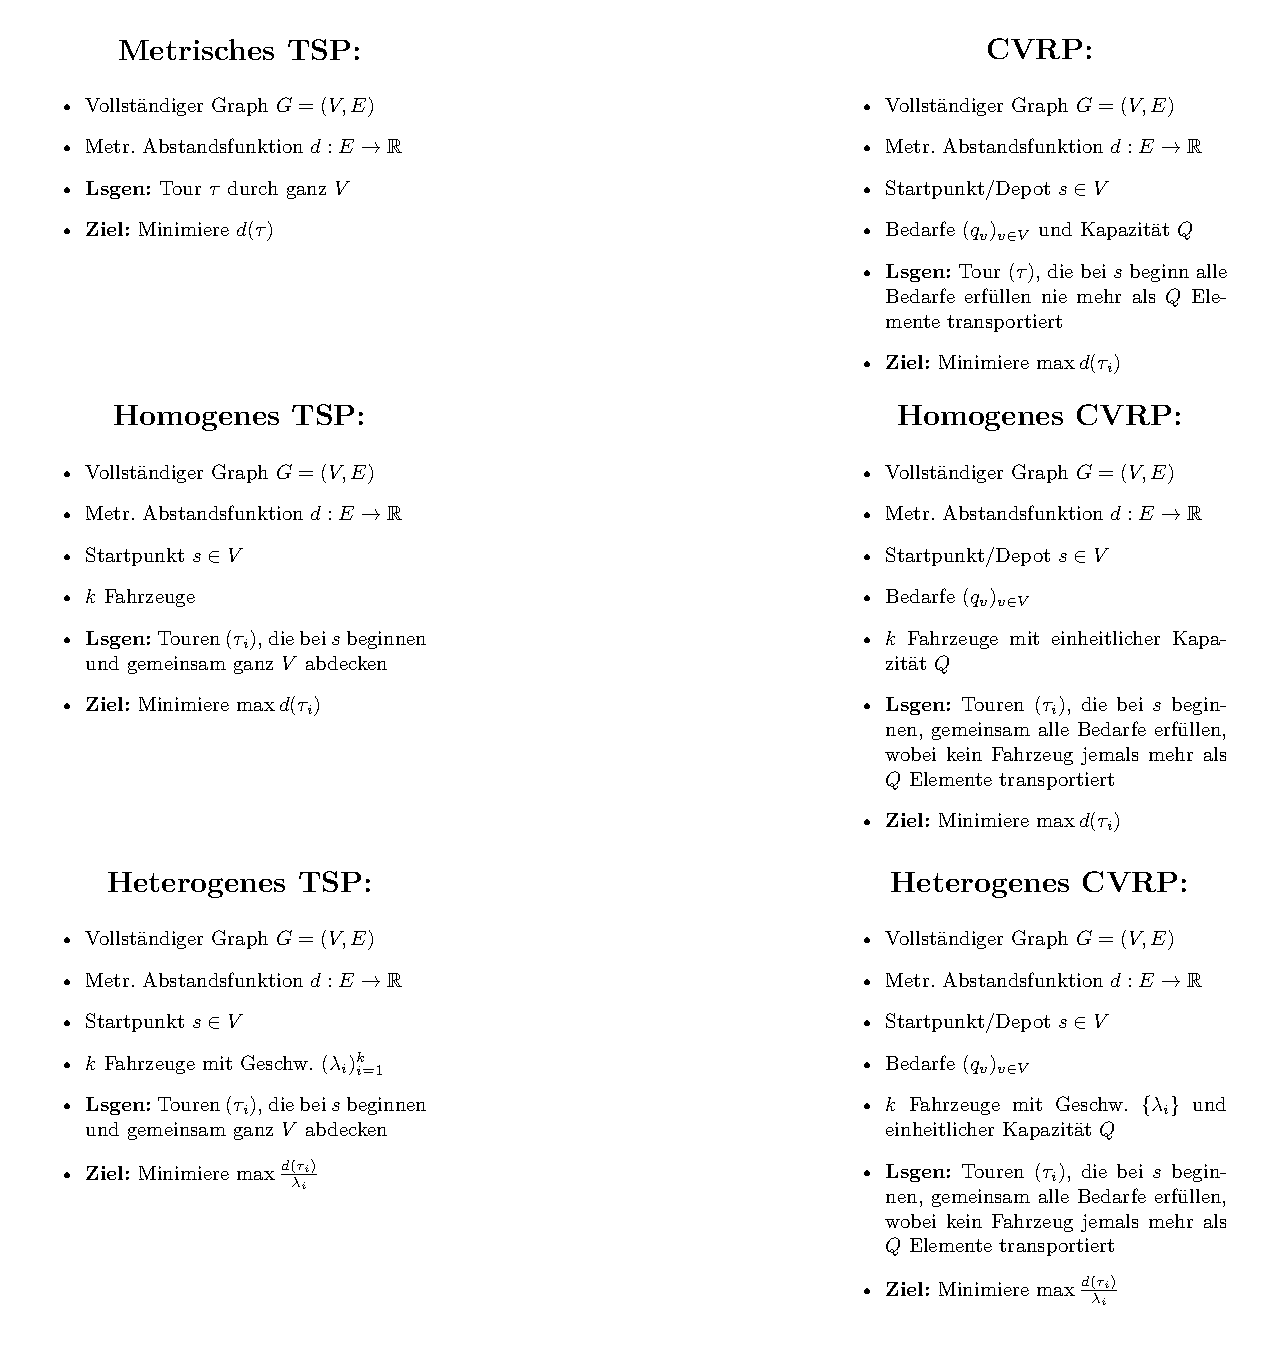
\includegraphics[width=1\textwidth]{Problemdefinitionen.pdf}
	
	\newpage
	\section{Algorithmen für \HomTSP und \CVRP}

	\subsection*{Vorbemerkungen}
	
	Verwendet folgende Konvention: Eine Funktion $f: M \to \RR$ induziert Funktionen 
	\[\tilde{f}: \mathcal{P}(M) \to \RR: N \mapsto \sum_{m\in N} f(m) \]
	und 
	\[\hat{f}_n: \prod_{i=1}^n M \to \RR: (m_i) \mapsto \sum_{i=1}^n f(m_i). \]
	die wir unter Überladung der Notation ebenfalls mit $f$ bezeichnen werden.
	
	
	\newpage
	\subsection{Algorithmus für \HomTSP}

	\begin{algorithm}[H]
		\caption{HomTSP-Approx}\label{AlgHomTSP}
		\begin{algorithmic}[1]
			\Procedure{HomTSP}{$G=(V,E)$, $d:E\to \RR_{\geq 0}, k$}
			\State $\tau \gets$ \textsc{TSP-Approx} $\left(G, d\right)$
			\State $\left(\pi_i\right)_{i=1}^k \gets$ Teile $\tau$ durch Entfernen von Kanten in $k$ Teilstrecken mit Länge $\leq \frac{d(\tau)}{k}$
			\State $\left(\tau_i\right)_{i=1}^k \gets$ Verbinde die zwei Endpunkte von $\pi_i$ mit $s$.
			\State \Return $\left(\tau_i\right)$
			\EndProcedure
		\end{algorithmic}
	\end{algorithm}	
	
	\begin{lemma}[Theorem 8 in \cite{TourSpliting}\footnote{Tatsächlich wird in \cite{TourSpliting} mit einem etwas komplexeren Algorithmus sogar eine Approximationsgüte von $\rho + 1 - \frac{1}{k}$ erreicht.}]
		Unter Verwendung eines $\rho$-approximativen Algorithmus (z.B. $\rho=\frac{3}{2}$ durch Christofides) für \TSP{} ist \textsc{HomTSP} $(\rho+1)$-approximativ.
	\end{lemma}
	
	\begin{proof}
		Schritt 3 ist möglich, denn jeder Pfad~$\pi_i$ entspricht Kanten der Gesamtlänge~${>\frac{d(\tau)}{k}}$ in $\tau$: Zunächst die (möglicherweise 0 vielen) Kanten in $pi_i$ der Gesamtlänge~$\leq \frac{d(\tau)}{k}$ und dann der entfernten nächsten Kante, die die Gesamtlänge über diese Schwelle gebracht hätte. Nach dem Erstellen der ersten $(k-1)$ Pfade sind daher höchstens noch Kanten der Länge 
			\[d(\tau) - \sum_{i=1}^{k-1}d(\pi_i) < d(\tau) - (k-1)\cdot \frac{d(\tau)}{k} = \frac{d(\tau)}{k}\]
		übrig, die daher von $\pi_k$ abgedeckt werden können.
		
		Da jeder der Endpunkte $u$ und $v$ von $\pi_i$ auch in einer optimalen Lösung besucht werden muss, gilt sicher $d(s,u), d(s,v) \leq \frac{1}{2}\OPT_\HomTSP$. Außerdem ist die Vereinigung aller Touren $\tau_i^\ast$ einer optimalen Lösung von \HomTSP{} eine zulässige Lösung von $\TSP$ und damit $\OPT_\TSP \leq \sum_{i=1}^{k}d(\tau_i^\ast) \leq k\cdot \max_{i=1}^{k}d(\tau_i^\ast) = k\cdot \OPT_\HomTSP$.
		
		Zusammen ergibt dies für jede der Touren $\tau_i$ (und damit insbesondere für die längste):
		\begin{align*}
			d(t_i) &\leq \frac{d(\tau)}{k} + 1\cdot \OPT_\HomTSP \leq \frac{\rho\cdot \OPT_\TSP}{k} + \OPT_\HomTSP \\
			       &\leq \frac{\rho\cdot k\cdot \OPT_\HomTSP}{k} + \OPT_\HomTSP = (\rho+1) \OPT_\HomTSP)
		\end{align*}
	\end{proof}
	
	
	\newpage
	\subsection{Algorithmus für \CVRP}
	
	\begin{algorithm}[H]
		\caption{CVRP-Approx}\label{AlgCVRP}
		\begin{algorithmic}[1]
			\Procedure{CVRP}{$G=(V,E)$, $d:E\to \RR_{\geq 0}, Q, (q_v)_{v\in V}$}
			\State $G' \gets$ vollst. Graph auf $V' := \left\lbrace v^{(j)} \mid v \in V, j=1,\dots,q_v\right\rbrace$
			\State $d'(v^{(i)}, u^{(j)}) := d(v,u)$
			\State $\tau \gets$ \textsc{TSP-Approx} $\left(G', d'\right)$
			\For{$v \in V'$}
				\State $\left(\pi_r^{(v)}\right) \gets$ Teile $\tau$ durch Kantenlöschen in Teilstrecken mit max. $Q$ Knoten,
				\Statex \hspace{8em} wobei die erste Strecke bei $v$ beginnt.
				\State $\left(\sigma_r^{(v)}\right) \gets$ Verbinde die zwei Endpunkte von $\pi^{(v)}_r$ mit $s$.
			\EndFor
			\State $\left(\sigma_r\right) \gets \left(\sigma_r^{(v)}\right)$ mit $\sum_r d'(\sigma_r^{(v)})$ minimal.
			\State \Return $\left(\sigma_r\right)$
			\EndProcedure
		\end{algorithmic}
	\end{algorithm}	
	
	\begin{prop}[Lemma 1 in \cite{CVRPApprox}]\label{CVRPLowerBound}
		Es gilt: 
			\[\OPT_\CVRP \geq \max\left\lbrace\OPT_\TSP, \frac{2}{Q}\sum_{v'\in V'}d'(s,v')\right\rbrace\]
	\end{prop}
	
	\begin{proof}
		Die erste Abschätzung ist klar (eine \CVRP-Route ist insbesondere auch eine \TSP-Tour).
		
		Für die zweite Abschätzung betrachte eine optimale Route $\left(\sigma_r^\ast\right)$, wobei $S_r \subseteq V'$ die in der $r$-ten Tour besuchten Knoten seien. Dann gilt offenbar:
			\[d\left(\sigma_i^\ast\right) \geq 2\cdot \max\left\lbrace d(s,v') \mid v'\in S_r\right\rbrace \geq 2\frac{\sum_{v'\in V'}d(s,v')}{\left|S_r\right|} \geq \frac{2}{Q}\sum_{v'\in S_r}d(s,v')\]
		
		Da jeder Knoten aus $V'$ in wenigstens einem $S_r$ enthalten sein muss, folgt damit:
			\[\OPT_\CVRP = \sum_r d\left(\sigma_i^\ast\right) \geq \frac{2}{Q}\sum_r\sum_{v'\in S_r}d(s,v') \geq \frac{2}{Q}\sum_{v'\in V'}d(s,v')\]
	\end{proof}
	
	\begin{lemma}[Lemma 2 in \cite{CVRPApprox}\footnote{Wie über eine genauere Abschätzung in \cite{CVRPApprox} gezeigt wird, erreicht der Algorithmus sogar eine Approximationsgüte von $\rho + \lceil\frac{n'}{Q}\rceil \frac{Q-\rho}{n'}$, wobei $n' := \sum_v q_v$}]\label{AlgCVRPProof}
		Unter Verwendung eines $\rho$-approximativen Algorithmus für \TSP{} ist \textsc{CVRP-Approx} $(\rho+2)$-approximativ.
	\end{lemma}	
	
	\begin{proof}
		Sei $n' := \sum_v q_v = \left|V'\right|$ und $m := \lceil\frac{n'}{Q}\rceil$. Dann gilt für die Summe aller möglichen Routen:
			\[\sum_{v,r} d'(\sigma_r^{(v)}) \leq 2m\sum_{v'\in V'}d'(s,v') + n'\cdot d(\tau)\]
		Denn jeder Knoten ist genau einmal Anfangs- und einmal Endpunkt für jede der $m$ Teilstrecken (erster Summand) und jede Route entsteht durch Weglassen von Kanten aus der Tour $\tau$ (zweiter Summand).
		
		Die beste dieser Routen ist sicher mindestens so gut wie der Durchschnitt aus allen möglichen Routen, also:
			\[\sum_{r} d'(\sigma_r) = 2\frac{m}{n'}\sum_{v'\in V'}d'(s,v') + d(\tau) \leq 2\frac{\frac{n'}{Q}+1}{n'}\sum_{v'\in V'}d'(s,v')+ d(\tau) \leq  2\cdot\frac{2}{Q}\sum_{v'\in V'}d'(s,v') + \rho\cdot\OPT_\TSP\]
		Zusammen mit \Cref{CVRPLowerBound} ergibt dies:
			\[\sum_{r} d'(\sigma_r) \leq 2\cdot\OPT_\CVRP + \rho\cdot\OPT_\CVRP \leq \left(2+\rho\right)\cdot\OPT_\CVRP\]
	\end{proof}
	
	\section{Algorithmus für \HetTSP}
	
	\begin{algorithm}[H]
		\caption{HetTSP-Approx}\label{AlgHetTSP}
		\begin{algorithmic}[1]
			\Procedure{HetTSP}{$G=(V,E)$, $d:E\to \RR_{\geq 0}$}
			\State Rate $M$ mit $\OPT \leq M \leq 2\cdot\OPT$
			\State $\Hc := \left(H_l\right)_{l\geq 0} \gets$ \textsc{Level-Prime} $\left(G, d\right)$
			\Statex \Comment{$\Hc$ erfüllt: Wurzel-Blatt Pfade haben aufsteigende Knoten-Level}
			\Statex \Comment{\phantom{$\Hc$ erfüllt:} und $\forall l: \sum_{j\geq l}d\left(H_j\right)\leq 8 M \sum_{j\geq l-1}2^j\mu_j$ (wenn $M$ korrekt geraten)}
			\State $\Tc := \left(\Tc_i\right)_{i\geq 0} \gets$ \textsc{Decomposition} $\left(\Hc\right)$
			\Statex \Comment{$\Tc$ ist $\left(6, 40\right)$-zuweisbarer Wald}
			\State $\left(x_{ij}\right) \gets$ \textsc{FractionalAssignment}  $\left(\Tc\right)$
			\State $\left(\tau_i\right) \gets$ \textsc{RoundingAssignment} $\left(x_{ij}\right)$
			\Statex \Comment{$\Tc$ ist $\left(\alpha, \beta\right)$-zuweisbar $\Rightarrow$ $\left(\tau_i\right)$ ist $\left(4\alpha+2\beta\right)$-approx.}
			\State \Return $\left(\tau_i\right)$
			\EndProcedure
		\end{algorithmic}
	\end{algorithm}
	
	\begin{satz}[Theorem 1.1 in \cite{HetCVRP}]
		\Cref{AlgHetTSP} ist ein $\Oc(1)$-approximativer Algorithmus für \HetTSP.
	\end{satz}
	
	\begin{proof}
		Folgende Kapitel...
	\end{proof}
	
	\subsection{Level-Prime}
	
	\begin{algorithm}[H]
		\caption{Level-Prime}\label{AlgLevelPrime}
		\begin{algorithmic}[1]
			\Procedure{Level-Prime}{$G=(V,E)$, $d:E\to \RR_{\geq 0}$}
			\State $V_0 := \left\lbrace v\in V \mid d(s,v) \leq M\right\rbrace,\quad V_i := \left\lbrace v \in V \mid 2^{i-1}M < d(s,v) \leq 2^i M\right\rbrace$
			\LineFor{$i\geq 0$}{$H_i \gets$ Minimaler Spannbaum auf $G\left[V_{\leq i}\right]/V_{<i}$}
			\State \Return $\left(H_i\right)_{i\geq 0}$
			\EndProcedure
		\end{algorithmic}
	\end{algorithm}	
	
	\begin{lemma}[Theorem 3.3 in \cite{HetCVRP}]
		Ein von \cref{AlgLevelPrime} gefundener Baum $\left(H_l\right)_{l\geq 0}$ erfüllt:
		\begin{itemize}
			\item Die Knoten-Level entlang jedes Wurzel-Blatt-Pfades sind monoton wachsend.
			\item $\forall j\geq 0: \sum_{l\geq j} d(H_l) \leq 8\cdot \MST(G/V_{<j})$
		\end{itemize}
	\end{lemma}
	
	\begin{kor}[Korollar 3.5 in \cite{HetCVRP}]
		Ein von \cref{AlgLevelPrime} gefundener Baum $\left(H_l\right)_{l\geq 0}$ erfüllt:
		\begin{itemize}
			\item Die Knoten-Level entlang jedes Wurzel-Blatt-Pfades sind monoton wachsend.
			\item $\forall j\geq 1: \sum_{l>j} d(H_l) \leq 8M\cdot \sum_{l\geq j}2^l\mu_l$
		\end{itemize}
	\end{kor}
	
	
	\subsection{Zerlegungsalgorithmus}
	
	\begin{algorithm}[H]
		\caption{Decomposition}\label{AlgDecomposition}
		\begin{algorithmic}[1]
			\Procedure{Decomposition}{$\left(\Hc\right)$}
			\State $\Sc_0 := \left\lbrace H_0 \right\rbrace,\quad \Sc_l := \text{Zerl. von } \Hc\cap E_l \text{ in Bäume mit genau einer Kante nach } V_l$
			\State $\Sc_l^{\geq} := \left\{\tau \in \Sc_l \mid d(\tau) \geq 2^{l-3}M\right\}, \Sc_l^< := \Sc_l \backslash \Sc_l^{\geq}$
			\LineFor{$\tau \in \Sc_l^{<}$}{$h(\tau) := \tau' \in S_{l-1}^{\geq}$ mit $\tau \cup \tau'$ zsh. (ex. eind.)}
			\For{$\tau \in \Sc_l^{\geq}$}
				\State $\Tc_l(\tau) \gets$ Partition von $\tau \cup h^{-1}(\tau)$ in Bäume der Länge $\left[2^{l+1}M, 2^{l+2}M\right]$ 
				\Statex \hspace{6.5em} (und evtl. ein kürzerer)
				\State $\Tc'_l(\tau) \gets \left\{T_r \cup \{\text{kürzeste Kante zu } s\} \mid T_r \in \Tc_l(\tau)\right\}$
			\EndFor
			\State $\Tc_l := \bigcup_{\tau \in \Sc_l^{\geq}}\Tc'_l(\tau)$
			\State \Return $\left(\Tc_l\right)_{l\geq 0}$
			\EndProcedure
		\end{algorithmic}
	\end{algorithm}
	
	\begin{defn}[Definition 3.1 in \cite{HetCVRP}]
		Ein Wald $\Tc = \bigcup_{l\geq 0} \Tc_l$ aus Bäumen mit Wurzel $s$ heißt $(\alpha, \beta)$-zuweisbar, wenn gilt:
		\begin{itemize}
			\item Für alle $T \in \Tc_l$ gilt: $d(T) \leq \alpha 2^l M$ \\
			\textit{d.h. ein Baum aus $\Tc_l$ kann mit Geschw. $2^l$ in $\Oc(\alpha M)$ besucht werden.}
			\item Für alle $k \geq 1$ gilt: $\sum_{l > k} d(\Tc_l) \leq \beta M \sum_{l\geq k} 2^l\mu_l$
			
			\textit{d.h. die Fahrzeuge mit Geschw. $\geq 2^k$ können den Wald $\Tc_{>k}$ in $\Oc(\beta M)$ besuchen.}
		\end{itemize}
	\end{defn}
	
	\begin{lemma}[Lemma 3.11 in \cite{HetCVRP}]
		Die von \cref{AlgDecomposition} bestimmte Zerlegung $\Tc = (\Tc_i)_{i\geq 0}$ ist $(6, 40)$-zuweisbar.
	\end{lemma}
	
	
	\subsection{Assignment-Algorithmen}

	\begin{algorithm}[H]
		\caption{FractionalAssignment}\label{AlgFractionalAssignment}
		\begin{algorithmic}[1]
			\Procedure{FractionalAssignment}{$\left(\Tc\right)$}
			\State $L := \{T \in \Tc\},\quad b(T) := d(T)$, \quad $R := \{i \mid 1\leq i \leq k\},\quad b(i) := \beta M 2^{\lambda_i}$
			\State $F := \{\{T,i\} \mid T \in \Tc_l, \lambda_i \geq l-1\}$ 
			\State Bestimme $L$-überdeckendes $b$-Matching $x_{Ti}$.
			\State \Return $\left(x_{Ti}\right)$
			\EndProcedure
		\end{algorithmic}
	\end{algorithm}
	
	\begin{prop}[Seite 54 (?) in \cite{bMatching}]
		$b$-Matching existiert und kann mit Max-Flow in polynomieller Zeit gefunden werden.
	\end{prop}
	
	\begin{algorithm}
		\caption{RoundingAssignment}\label{AlgRoundingAssignment}
		\begin{algorithmic}[1]
			\Procedure{RoundingAssignment}{$\left(x_{Ti}\right)$}
			\State $\left(x'_{Ti}\right) \gets$ \textsc{RoundScheduling}($p_{Ti} := \frac{d(T)}{2^{\lambda_i}}, \tilde{x}_{Ti} := \frac{x_{Ti}}{d(T)}$)
			\State $\tau_i \gets$ Tour durch die Bäume $T$ mit $x'_{Ti} = 1$.
			\State \Return $\left(\tau_i\right)$
			\EndProcedure
		\end{algorithmic}
	\end{algorithm}
	
	\begin{prop}[Theorem 1 in \cite{Rounding}]
		Gegeben folgendes Scheduling-Problem: Job $T$ benötigt auf Maschine $i$ Zeit $p_{Ti}$. $J_i(t) := \{T \mid p_{Ti} \leq t\}$ und $M_T(t) := \{i \mid p_{Ti} \leq t\}$.
		
		Eine rationale Lösung $\tilde{x}_{Ti}$ mit
			\[\sum_{i\in M_T(t)} \tilde{x}_{Ti} = 1, \quad \sum_{T\in J_i(t)} p_{Ti}\tilde{x}_{Ti} \leq \beta M, \quad \tilde{x}_{Ti} \geq 0 \]		
		kann in polynomieller Zeit zu einer ganzen Lösung $x'_{Ti}$ gerundet werden mit:
			\[\sum_{i\in M_T(t)} x'_{Ti} = 1, \quad \sum_{T\in J_i(t)} p_{Ti} x'_{Ti} \leq \beta M + t, \quad x'_{Ti} \in \{0,1\} \]
	\end{prop}
	
	\begin{lemma}[Lemma 3.2 in \cite{HetCVRP}]
		Gegeben einen $(\alpha, \beta)$-zuweisbaren Wald, liefern \cref{AlgFractionalAssignment} und \cref{AlgRoundingAssignment} eine $(4\alpha+2\beta)$-approximative Lösung für \HetTSP.
	\end{lemma}
	
	\begin{proof}
		$\tilde{x}_{Ti}$ erfüllt:
			\[\sum_{i\in M_T(2\alpha M)} \tilde{x}_{Ti} = 1, \quad \sum_{T\in J_i(2\alpha M)} p_{Ti}\tilde{x}_{Ti} \leq \beta M, \quad \tilde{x}_{Ti} \geq 0 \]
		Somit gibt \Cref{AlgRoundingAssignment} eine Zuweisung mit 	
			\[\sum_{T\in J_i(t)} p_{Ti}\tilde{x}_{Ti} \leq \beta M + 2\alpha M\]
		Durch Verdoppeln der Kanten in den Bäumen, erhalten wir daraus Touren mit $d(\tau_i) \leq 2\cdot \left(\beta M + 2\alpha M\right)$.
	\end{proof}
	
	\section{Algorithmus für \HetCVRP}
	
	\begin{algorithm}[H]
		\caption{Reduktion}\label{AlgReduktion}
		\begin{algorithmic}[1]
			\Procedure{Reduktion}{$G=(V,E), d: E\to \mathbb{R}_{\geq 0}, s\in V, Q, (\lambda_i), (q_v)$}
			\State $V' := \left\lbrace v^{(j)} \mid v \in V, j=1,\dots,q_v\right\rbrace,\quad E' := \left\lbrace \{v^{(j)},v\} \mid v \in V, j=1,\dots,q_v\right\rbrace$
			\State $\tilde{G} := (V\cup V', E\cup E'), \quad\quad\quad\quad\quad\quad \tilde{d}(v^{(j)},v) := \frac{d(s,v)}{Q}$, sonst wie $d$
			\State \Return $\left(\tilde{G}, \tilde{d}, s, Q, (\mu_i)\right)$
			\EndProcedure
		\end{algorithmic}
	\end{algorithm}	
	
	\begin{lemma}
		Für jede Instanz $\Ic$ von \HetCVRP{} ist $\Jc := \textsc{Reduktion}(\Ic)$ eine Instanz von \HetTSP{} mit:
			\[\OPT_\HetTSP(\Jc) \in \Oc(1)\cdot\OPT_\HetCVRP(\Ic)\]
	\end{lemma}
	
	\begin{proof}
		Sei $(\sigma_i)$ eine optimale Lösung von $\Ic$. Definiere $c_i(v) := \#\text{Einheiten von }i\text{ an }v\text{ geliefert}$. Dann gilt also:
			\[\sum_i c_i(v) = q_v, \text{ für alle } v \in V\]
		Folglich ist es möglich $U'_i \subseteq V'$ zu wählen, sodass gilt
			\[\bigcup_i U'_i = V' \text{ und } \left|\left\lbrace v^{(j)} \in U'_i \right\rbrace\right| = c_i(v)\]
		Definiere weiter $U_i := \left\lbrace v \in V \mid v^{(j)} \in U'_i\right\rbrace$.
		
		Seien nun $\tau_i$ minimale \TSP-Touren durch $U'_i \cup U_i \cup \{s\}$. Zusammen sind diese dann insbesondere eine zulässige Lösung für die \HetTSP-Instanz $\Jc$ und es gilt:
		\begin{align*}
			d(\tau_i) &\leq 2\cdot \MST(U'_i \cup \{s\}) = 2\cdot \left(\MST(U_i \cup \{s\}) + \sum_{v' \in U'_i} \tilde{d}(v,v')\right) \\
					  &= 2\cdot \left(\MST(U_i \cup \{s\}) + \sum_{v \in U_i}c_i(v)\frac{d(s,v)}{Q}\right) \leq 2\cdot \left(d(\sigma_i) + d(\sigma_i)\right) = 4 \cdot d(\sigma_i)
		\end{align*}
		Die erste Abschätzung gilt, da man eine zulässige Tour erhalten kann, indem man einen minimalen Spannbaum nimmt, alle Kanten verdoppelt und dann eine Eulertour bestimmt. Bei der zweiten Abschätzung ist:
		\begin{itemize}
			\item $\MST(U_i \cup \{s\}) \leq d(\sigma_i)$, denn $\sigma_i$ besucht alle Knoten in $U_i$, enthält also insbesondere einen Spannbaum von $U_i \cup \{s\}$.
			\item $\sum_{v \in U_i}c_i(v)\frac{d(s,v)}{Q} \leq d(\sigma_i)$, denn $\sigma_i$ ist eine zulässige Lösung für das \CVRP-Problem auf $U_i$ mit Bedarfen $c_i(v)$. Damit folgt die Ungleichung aus \Cref{CVRPLowerBound}.
		\end{itemize}
		
		Insgesamt folgt daher:
			\[\OPT_\HetTSP(\Jc) \leq \max d(\tau_i) \leq 4\cdot \max d(\sigma_i) = 4\cdot \OPT_\HetCVRP(\Ic)\]
	\end{proof}

	\begin{algorithm}[H]
		\caption{Deduktion}\label{AlgDeduktion}
		\begin{algorithmic}[1]
			\Procedure{Deduktion}{$\Ic, \Jc, (\tau_i)$}
			\For{$i \gets 1, \dots, k$}
				\State $c_i(v) := \left|\left\lbrace v^{(j)} \mid v^{(j)} \in \tau_i \right\rbrace\right|$
				\State $\sigma_i \gets $ \textsc{CVRP-Approx}($G, d, Q, \left(c_i(v)\right)_{v\in V}$)
			\EndFor
			\State \Return $\left(\sigma_i\right)$
			\EndProcedure
		\end{algorithmic}
	\end{algorithm}	
	
	\begin{lemma}
		Für jede Lösung $(\tau_i)$ von $\Jc$ ist $(\sigma_i)$ eine Lösung von $\Ic$ mit:
		\[\max \frac{d(\sigma_i)}{\lambda_i} \in \Oc(1)\cdot \max \frac{d(\tau_i)}{\lambda_i}\]
	\end{lemma}
	
	\begin{proof}
		Nach \Cref{AlgCVRPProof} liefert \Cref{AlgCVRP} eine Lösung mit 
			\[d(\sigma_i) \leq \rho\cdot \OPT_\TSP(U'_i, d) + \frac{2}{Q}\sum_{v'\in U'_i}d'(s,v')\]
		Ferner ist
			\[\OPT_\TSP(U'_i, d) \leq d(\tau_i) \text{ und } \frac{2}{Q}\sum_{v'\in U'_i}d'(s,v') \leq d(\tau_i)\]
		Also zusammen
			\[d(\sigma_i) \leq (\rho + 1) \cdot d(\tau_i)\]		
	\end{proof}	
	
	\begin{satz}[Theorem 4.1 in \cite{HetCVRP}]
		Es gibt eine $\Oc(1)$-approximationserhaltende Reduktion von \HetTSP{} auf \HetCVRP.
	\end{satz}
	
	\begin{proof}
		Verwende \Cref{AlgReduktion} um die Eingabe zu einer Instanz von \HetTSP{} zu machen. Finde eine $\Oc(1)$-approximative Lösung für diese mit Hilfe von \Cref{AlgHetTSP}. Schließlich erhalte aus dieser mit \Cref{AlgDeduktion} eine Lösung der \HetCVRP-Instanz.

		Für diese Lösung gilt:
		
		 \[\max \frac{d(\sigma_i)}{\lambda_i} \in \Oc(1)\cdot \max \frac{d(\tau_i)}{\lambda_i} \subseteq \Oc(1)\cdot\OPT_\HetTSP(\Jc) \subseteq \Oc(1)\cdot\OPT_\HetCVRP(\Ic)\]
	\end{proof}

	\newpage
	\nocite{*}
	\printbibliography		
			
\end{document}